% Supplementary theory, experiments, and implementation details.

\section{Regularity of the Hopfield Energy}
\subsection{Proof of Proposition~\ref{prop:regularity}}\label{app:proof-regularity}

We prove the two regularity properties of the modern Hopfield energy $E$ defined in~\eqref{eq:modern-hopfield-energy}. Write $\mathbf{p}(\boldsymbol{\xi})=\operatorname{softmax}(\beta\mathbf{X}^{\top}\boldsymbol{\xi}+\log\mathbf r)\in\mathbb{R}^K$ for the attention weight vector at state $\boldsymbol{\xi}$, restricted to the support where $r_k>0$, and recall the retrieval map $\mathbf{T}(\boldsymbol{\xi})=\mathbf{X}\mathbf{p}(\boldsymbol{\xi})$.

\paragraph{Hessian computation.}
The gradient is $\nabla E(\boldsymbol{\xi})=\boldsymbol{\xi}-\mathbf{T}(\boldsymbol{\xi})$~\cite{ramsauerHopfieldNetworksAll2021}. To obtain the Hessian we differentiate the retrieval map. Let $\mathbf{z}=\beta\mathbf{X}^{\top}\boldsymbol{\xi}\in\mathbb{R}^K$ denote the pre-softmax logits. The softmax has the following $K\times K$ Jacobian:
\begin{equation}\label{eq:softmax-jacobian}
    \frac{\partial\mathbf{p}}{\partial\mathbf{z}}
    = \operatorname{diag}(\mathbf{p}) - \mathbf{p}\mathbf{p}^{\top}
    =: \mathbf{S}(\mathbf{p}),
\end{equation}
This Jacobian is the covariance matrix of a categorical distribution with
probabilities $\mathbf p$. The chain rule gives the Hessian:
\begin{equation}\label{eq:hessian}
    \nabla^{2}E(\boldsymbol{\xi})
    = \mathbf{I}_{d} - \beta\,\mathbf{X}\,\mathbf{S}\bigl(\mathbf{p}(\boldsymbol{\xi})\bigr)\,\mathbf{X}^{\top}.
\end{equation}

\paragraph{Part (i): Lipschitz gradient.}
The Lipschitz constant of $\nabla E$ equals $\sup_{\boldsymbol{\xi}}\|\nabla^{2}E(\boldsymbol{\xi})\|_{\mathrm{op}}$. Because $\mathbf{S}(\mathbf{p})$ is a covariance matrix it is positive semidefinite, so $\beta\mathbf{X}\mathbf{S}\mathbf{X}^{\top}\succeq\mathbf{0}$. The triangle inequality for the spectral norm gives:
\begin{equation}\label{eq:lip-triangle}
    \|\nabla^{2}E(\boldsymbol{\xi})\|_{\mathrm{op}}
    \;\le\; \|\mathbf{I}_{d}\|_{\mathrm{op}}
            + \beta\,\|\mathbf{X}\,\mathbf{S}(\mathbf{p})\,\mathbf{X}^{\top}\|_{\mathrm{op}}
    \;\le\; 1 + \beta\,\sigma_{\max}^{2}\,\|\mathbf{S}(\mathbf{p})\|_{\mathrm{op}},
\end{equation}
where the second step uses submultiplicativity of the spectral norm.

It remains to bound $\|\mathbf{S}(\mathbf{p})\|_{\mathrm{op}}$. For any unit vector $\mathbf{v}\in\mathbb{R}^K$, the quadratic form is:
\begin{align*}
\mathbf{v}^{\top}\mathbf{S}(\mathbf{p})\mathbf{v}
= \sum_{i}p_{i}v_{i}^{2} - \Bigl(\sum_{i}p_{i}v_{i}\Bigr)^{\!2}
= \operatorname{Var}_{\mathbf{p}}(V),
\end{align*}
Here $V$ is the random variable taking value $v_i$ with probability $p_i$. By Popoviciu's variance inequality, $\operatorname{Var}(V)\le(v_{\max}-v_{\min})^{2}/4$. Under the constraint $\|\mathbf{v}\|_{2}=1$, its range satisfies:
\begin{align*}
(v_{\max}-v_{\min})^{2}
\;\le\; (|v_{\max}|+|v_{\min}|)^{2}
\;\le\; 2(v_{\max}^{2}+v_{\min}^{2})
\;\le\; 2\|\mathbf{v}\|_{2}^{2} = 2,
\end{align*}
The second step is the Cauchy--Schwarz inequality
$(a+b)^{2}\le 2(a^{2}+b^{2})$ for $a,b\ge 0$. Therefore, the softmax
covariance obeys the bound:
\begin{equation}\label{eq:softmax-spectral-bound}
    \|\mathbf{S}(\mathbf{p})\|_{\mathrm{op}}
    = \sup_{\|\mathbf{v}\|=1}\operatorname{Var}_{\mathbf{p}}(V)
    \;\le\; \frac{2}{4} = \frac{1}{2},
\end{equation}
and this bound is tight: equality holds when $K\ge 2$ with $\mathbf{p}=(\tfrac{1}{2},\tfrac{1}{2},0,\dots,0)$ and $\mathbf{v}=(\tfrac{1}{\sqrt{2}},-\tfrac{1}{\sqrt{2}},0,\dots,0)$.

Substituting Eq.~\eqref{eq:softmax-spectral-bound} into
Eq.~\eqref{eq:lip-triangle} gives the Lipschitz constant:
\begin{align*}
\sup_{\boldsymbol{\xi}}\|\nabla^{2}E(\boldsymbol{\xi})\|_{\mathrm{op}}
\;\le\; 1 + \frac{\beta\,\sigma_{\max}^{2}}{2}
=: L.
\end{align*}

\paragraph{Part (ii): Dissipativity.}
Expanding the inner product gives:
\begin{align*}
\langle\nabla E(\boldsymbol{\xi}),\,\boldsymbol{\xi}\rangle
= \|\boldsymbol{\xi}\|_{2}^{2} - \langle\mathbf{T}(\boldsymbol{\xi}),\,\boldsymbol{\xi}\rangle.
\end{align*}
The retrieval map $\mathbf{T}(\boldsymbol{\xi})=\mathbf{X}\mathbf{p}=\sum_{k}p_{k}\mathbf{m}_{k}$ is a convex combination of stored patterns. The triangle inequality gives:
\begin{align*}
\|\mathbf{T}(\boldsymbol{\xi})\|_{2}
= \Bigl\|\sum_{k}p_{k}\mathbf{m}_{k}\Bigr\|_{2}
\le \sum_{k}p_{k}\|\mathbf{m}_{k}\|_{2}
\le M,
\end{align*}
Here $M=\max_{k}\|\mathbf{m}_{k}\|_{2}$ and $\sum_{k}p_{k}=1$. The
Cauchy--Schwarz inequality gives:
\begin{align*}
|\langle\mathbf{T}(\boldsymbol{\xi}),\,\boldsymbol{\xi}\rangle|
\le \|\mathbf{T}(\boldsymbol{\xi})\|_{2}\,\|\boldsymbol{\xi}\|_{2}
\le M\|\boldsymbol{\xi}\|_{2}.
\end{align*}
Applying Young's inequality $ab\le\tfrac{a^{2}}{2}+\tfrac{b^{2}}{2}$ with $a=M$ and $b=\|\boldsymbol{\xi}\|_{2}$ gives:
\begin{align*}
M\|\boldsymbol{\xi}\|_{2}
\;\le\; \frac{M^{2}}{2} + \frac{\|\boldsymbol{\xi}\|_{2}^{2}}{2}.
\end{align*}
Combining these inequalities establishes dissipativity:
\begin{align*}
\langle\nabla E(\boldsymbol{\xi}),\,\boldsymbol{\xi}\rangle
\;\ge\; \|\boldsymbol{\xi}\|_{2}^{2} - \frac{M^{2}}{2} - \frac{\|\boldsymbol{\xi}\|_{2}^{2}}{2}
= \frac{1}{2}\|\boldsymbol{\xi}\|_{2}^{2} - \frac{M^{2}}{2},
\end{align*}
which is the dissipativity condition \textbf{(R2)} with constants $a=\tfrac{1}{2}$ and $b=\tfrac{M^{2}}{2}$. \qed

\paragraph{Sufficient convexity condition.}
Since $\mathbf{S}(\mathbf{p})\succeq\mathbf{0}$, the Hessian~\eqref{eq:hessian} satisfies $\nabla^{2}E\preceq\mathbf{I}$ (the identity provides an upper bound on the eigenvalues). Equation~\eqref{eq:softmax-spectral-bound} and submultiplicativity give the following lower bound:
\begin{align*}
\nabla^{2}E(\boldsymbol{\xi})
\;\succeq\; \Bigl(1-\frac{\beta\sigma_{\max}^{2}}{2}\Bigr)\mathbf{I}.
\end{align*}
When $\beta\sigma_{\max}^{2}<2$ the lower bound is strictly positive, so $E$ is strictly convex. The potential $U=\beta E$ is then $m$-strongly convex with $m=\beta(1-\beta\sigma_{\max}^{2}/2)$ and has $L_{U}$-Lipschitz gradient with $L_{U}=\beta(1+\beta\sigma_{\max}^{2}/2)$. Its condition number is:
\begin{align*}
\kappa = \frac{L_{U}}{m}
= \frac{1+\beta\sigma_{\max}^{2}/2}{1-\beta\sigma_{\max}^{2}/2},
\end{align*}
which diverges as the sufficient lower bound approaches zero. This bound does
not locate the exact onset of nonconvexity or count local minima.




\section{Additional Experiments and Diagnostics}
\label{app:additional-experiments}

The experiments in this section provide qualitative inspection and
reproducibility details. Unless an
exact all-component row is shown in the main text, they characterize the
finite-time, warm-started protocol rather than independent equilibrium
sampling. Novelty, diversity, and Hopfield energy are descriptive quantities;
they are not a cross-model quality ranking. Reported standard errors group
endpoints across 30 chains and should not be interpreted as uncertainty across
independent repetitions of the complete experiment.

\subsection{Synthetic responsibility concentration}
The load-ratio sweep remains useful as a finite-dimensional visualization of
attention-responsibility concentration. Its empirical contour is not a storage
capacity boundary or an automatic temperature selector.
\begin{figure}[t]
\centering

\includegraphics[width=0.65\textwidth]{figs/Fig_experiment-3-load-ratio.pdf}
\caption{Phase diagram of attention concentration $C = 1 - H(\mathbf{a})/\log K$ over load ratio $K/d$ (horizontal; equivalently $\alpha=\log K/d\in[0.017,0.076]$, the capacity-relevant parameter for an exponential-capacity energy) and inverse temperature $\beta$ (vertical, log~scale), with $d=64$. Each cell averages over five independent datasets. The dashed contour marks $C=0.5$, separating a concentrated regime (upper-left, warm colors) from a diffuse regime (lower-right, dark colors). The contour is a finite-$d$ crossover proxy for the random-energy-model condensation line of Lucibello and M\'ezard~\cite{lucibelloExponentialCapacityDense2024}, not a measurement of storage capacity.}
\label{fig:phase-diagram}
\end{figure}

\subsection{MNIST baseline record}
\label{app:mnist-baseline-record}
Table~\ref{tab:mnist-baselines} reports the finite-time numerical comparison
alongside the exact-sampling analysis in the main text. The columns describe
endpoint geometry under different procedures.
They do not establish that one method is a better image generator.
\begin{table}[t]
\centering
\caption{MNIST digit-3 endpoint statistics ($K=100$, $d=784$).
Novelty, diversity, and Hopfield energy are descriptive geometry, not a quality
ranking. Values use the mean $\pm$ SE grouping across 30 chains.
$^\dagger$Energy is evaluated under the Hopfield target at $\beta=200$.}
\label{tab:mnist-baselines}
\small
\begin{tabular}{@{}lccc@{}}
\toprule
Method & $\mathcal{N}$ & $\bar{\mathcal{D}}$ & $\bar{E}$ \\
\midrule
Bootstrap (replay)          & $0.000 \pm 0.000$ & $0.459 \pm 0.011$ & $-0.500 \pm 0.000$ \\
Gaussian perturbation       & $0.004 \pm 0.000$ & $0.450 \pm 0.013$ & $-0.496 \pm 0.000$ \\
Random convex combination   & $0.092 \pm 0.000$ & $0.008 \pm 0.000$ & $-0.399 \pm 0.000$ \\
GMM-PCA ($r{=}50$, $C{=}10$) & $0.198 \pm 0.004$ & $0.419 \pm 0.011$ & $-0.303 \pm 0.005$ \\
VAE (latent${=}8$)          & $0.214 \pm 0.005$ & $0.441 \pm 0.008$ & $-0.286 \pm 0.005$ \\
MALA ($\beta{=}2000$)       & $0.151 \pm 0.001$ & $0.598 \pm 0.001$ & $-0.305 \pm 0.001$ \\
ULA ($\beta{=}2000$) & $0.152 \pm 0.001$ & $0.600 \pm 0.001$ & $-0.303 \pm 0.001$ \\
ULA ($\beta{=}200$) & $0.548 \pm 0.002$ & $0.885 \pm 0.002$ & $1.467 \pm 0.008^\dagger$ \\
\bottomrule
\end{tabular}
\end{table}

\subsection{Additional MNIST digits and temperature sweep}
Digits 1 and 8 test whether the endpoint behavior was specific to digit 3. The
images and tables are descriptive sensitivity analyses.
The broadening with decreasing $\beta$ is predicted directly by the exact
component width $\beta^{-1/2}$; visual degradation at low $\beta$ is important
context for interpreting increases in novelty and diversity.
\begin{table}[ht]
\centering
\caption{Quantitative comparison on MNIST digit ``1'' ($K{=}100$, $d{=}784$, $\beta{=}2000$). The protocol matches Table~\ref{tab:mnist-baselines}, including the VAE baseline (latent dimension 8, same two-phase training). The MALA acceptance rate was 99.2\%. Values are mean $\pm$ SE across 30 chains.}
\label{tab:mnist-digit1}
\small
\begin{tabular}{@{}lccc@{}}
\toprule
Method & $\mathcal{N}$ & $\bar{\mathcal{D}}$ & $\bar{E}$ \\
\midrule
Bootstrap (replay)          & $0.000 \pm 0.000$ & $0.416 \pm 0.019$ & $-0.500 \pm 0.000$ \\
Gaussian perturbation       & $0.004 \pm 0.000$ & $0.422 \pm 0.017$ & $-0.496 \pm 0.000$ \\
Random convex combination   & $0.097 \pm 0.001$ & $0.007 \pm 0.000$ & $-0.398 \pm 0.001$ \\
GMM-PCA ($r{=}50$, $C{=}10$) & $0.130 \pm 0.005$ & $0.401 \pm 0.017$ & $-0.366 \pm 0.005$ \\
VAE (latent${=}8$)          & $0.180 \pm 0.006$ & $0.408 \pm 0.008$ & $-0.320 \pm 0.006$ \\
MALA                        & $0.151 \pm 0.001$ & $0.586 \pm 0.001$ & $-0.305 \pm 0.001$ \\
ULA & $0.153 \pm 0.001$ & $0.591 \pm 0.001$ & $-0.303 \pm 0.001$ \\
\bottomrule
\end{tabular}
\end{table}

\begin{table}[ht]
\centering
\caption{Quantitative comparison on MNIST digit ``8'' ($K{=}100$, $d{=}784$, $\beta{=}2000$). The protocol matches Table~\ref{tab:mnist-baselines}, including the VAE baseline (latent dimension 8, same two-phase training). The MALA acceptance rate was 99.2\%. Values are mean $\pm$ SE across 30 chains.}
\label{tab:mnist-digit8}
\small
\begin{tabular}{@{}lccc@{}}
\toprule
Method & $\mathcal{N}$ & $\bar{\mathcal{D}}$ & $\bar{E}$ \\
\midrule
Bootstrap (replay)          & $0.000 \pm 0.000$ & $0.421 \pm 0.012$ & $-0.500 \pm 0.000$ \\
Gaussian perturbation       & $0.004 \pm 0.000$ & $0.450 \pm 0.011$ & $-0.496 \pm 0.000$ \\
Random convex combination   & $0.099 \pm 0.000$ & $0.007 \pm 0.000$ & $-0.395 \pm 0.000$ \\
GMM-PCA ($r{=}50$, $C{=}10$) & $0.194 \pm 0.005$ & $0.420 \pm 0.011$ & $-0.305 \pm 0.005$ \\
VAE (latent${=}8$)          & $0.209 \pm 0.005$ & $0.397 \pm 0.009$ & $-0.291 \pm 0.005$ \\
MALA                        & $0.151 \pm 0.001$ & $0.554 \pm 0.002$ & $-0.305 \pm 0.001$ \\
ULA & $0.152 \pm 0.001$ & $0.557 \pm 0.001$ & $-0.303 \pm 0.001$ \\
\bottomrule
\end{tabular}
\end{table}

\begin{figure}[ht]
\centering
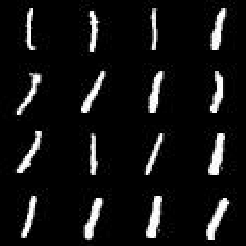
\includegraphics[width=0.19\textwidth]{figs/Fig_mnist_grid_bootstrap_digit1.pdf}%
\hfill
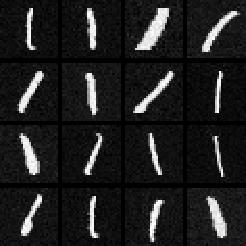
\includegraphics[width=0.19\textwidth]{figs/Fig_mnist_grid_gaussian_digit1.pdf}%
\hfill
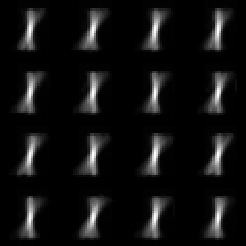
\includegraphics[width=0.19\textwidth]{figs/Fig_mnist_grid_convex_digit1.pdf}%
\hfill
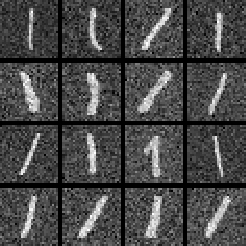
\includegraphics[width=0.19\textwidth]{figs/Fig_mnist_grid_mala_digit1.pdf}%
\hfill
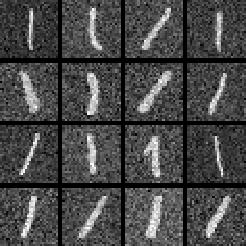
\includegraphics[width=0.19\textwidth]{figs/Fig_mnist_grid_sa_digit1.pdf}

\small
\makebox[0.19\textwidth]{\centering (a) Bootstrap}%
\hfill
\makebox[0.19\textwidth]{\centering (b) Gaussian}%
\hfill
\makebox[0.19\textwidth]{\centering (c) Convex}%
\hfill
\makebox[0.19\textwidth]{\centering (d) MALA}%
\hfill
\makebox[0.19\textwidth]{\centering (e) ULA}
\caption{MNIST digit-1 endpoint grids. The panels permit qualitative
inspection of replay, the narrow one-step Gaussian baseline, convex mixing,
MALA, and ULA. They are not an external image-quality evaluation.}
\label{fig:mnist-digit1-grids}
\end{figure}

\begin{figure}[ht]
\centering
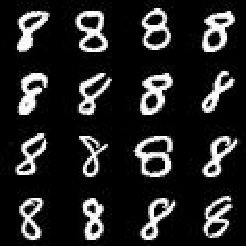
\includegraphics[width=0.19\textwidth]{figs/Fig_mnist_grid_bootstrap_digit8.pdf}%
\hfill
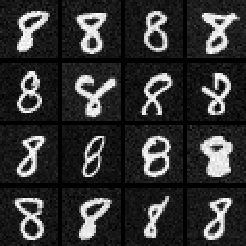
\includegraphics[width=0.19\textwidth]{figs/Fig_mnist_grid_gaussian_digit8.pdf}%
\hfill
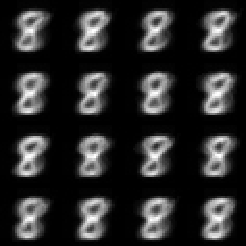
\includegraphics[width=0.19\textwidth]{figs/Fig_mnist_grid_convex_digit8.pdf}%
\hfill
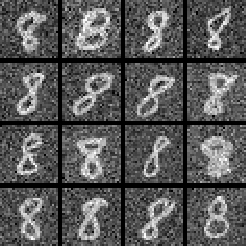
\includegraphics[width=0.19\textwidth]{figs/Fig_mnist_grid_mala_digit8.pdf}%
\hfill
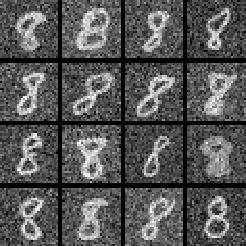
\includegraphics[width=0.19\textwidth]{figs/Fig_mnist_grid_sa_digit8.pdf}

\small
\makebox[0.19\textwidth]{\centering (a) Bootstrap}%
\hfill
\makebox[0.19\textwidth]{\centering (b) Gaussian}%
\hfill
\makebox[0.19\textwidth]{\centering (c) Convex}%
\hfill
\makebox[0.19\textwidth]{\centering (d) MALA}%
\hfill
\makebox[0.19\textwidth]{\centering (e) ULA}
\caption{MNIST digit-8 endpoint grids under the same finite-time
protocol as digit 1. These images show method-specific endpoint geometry but do
not establish a quality ordering.}
\label{fig:mnist-digit8-grids}
\end{figure}

\begin{table}[ht]
\centering
\caption{Temperature spectrum for digit 8 ($K=100$, $d=784$,
$\alpha=0.01$, 30 chains). The per-step SNR is the update ratio
$\sqrt{\alpha\beta/(2d)}$. It is a heuristic under spherical, unit-norm
assumptions, not an automatic regime boundary. Values use the
mean $\pm$ SE grouping.}
\label{tab:temp-spectrum-digit8}
\small
\begin{tabular}{@{}rccccc@{}}
\toprule
$\beta$ & SNR & $\mathcal{N}$ & $\bar{\mathcal{D}}$ & $\bar{E}$ & Mean max-$\cos$ \\
\midrule
2000 & 0.113 & $0.152 \pm 0.001$ & $0.557 \pm 0.001$ & $-0.3 \pm 0.00$ & $0.848 \pm 0.001$ \\
200  & 0.036 & $0.547 \pm 0.002$ & $0.872 \pm 0.002$ & $1.5 \pm 0.01$  & $0.453 \pm 0.002$ \\
50   & 0.018 & $0.753 \pm 0.002$ & $0.965 \pm 0.002$ & $7.4 \pm 0.03$  & $0.247 \pm 0.002$ \\
10   & 0.008 & $0.870 \pm 0.003$ & $0.992 \pm 0.002$ & $38.6 \pm 0.16$ & $0.130 \pm 0.003$ \\
\bottomrule
\end{tabular}
\end{table}

\subsection{Single-chain and trajectory diagnostics}
These experiments isolate finite-time initialization and trajectory behavior.
They are relevant to stochastic attention as a transition kernel. In the base
case their equilibrium target is also available through independent mixture
sampling; under additional energy terms, the trajectory sampler is the general
construction.
\begin{table}[ht]
\centering
\caption{Single-chain and multi-chain endpoint statistics for digit 3
($K=100$, $d=784$, $\alpha=0.01$). The comparison separates variation caused
by allocating warm starts across memories from variation along one finite-time
trajectory.}
\label{tab:single-chain}
\small
\setlength{\tabcolsep}{4pt}
\resizebox{\textwidth}{!}{%
\begin{tabular}{@{}llccccc@{}}
\toprule
Protocol & $\beta$ & SNR & $\mathcal{N}$ & $\bar{\mathcal{D}}$ & $\bar{E}$ & Max-$\cos$ \\
\midrule
Multi-chain (30 chains) & 2000 & 0.113 & $0.152 \pm 0.001$ & $0.600 \pm 0.001$ & $-0.303 \pm 0.001$ & $0.848 \pm 0.001$ \\
Single-chain            & 2000 & 0.113 & $0.153 \pm 0.000$ & $0.282 \pm 0.001$ & $-0.300 \pm 0.000$ & $0.847 \pm 0.000$ \\
Single-chain            & 200  & 0.036 & $0.551 \pm 0.001$ & $0.796 \pm 0.002$ & $\phantom{-}1.5\phantom{0} \pm 0.0\phantom{0}$ & $0.449 \pm 0.001$ \\
Single-chain            & 50   & 0.018 & $0.756 \pm 0.002$ & $0.967 \pm 0.002$ & $\phantom{-}7.4\phantom{0} \pm 0.0\phantom{0}$ & $0.244 \pm 0.002$ \\
\bottomrule
\end{tabular}}
\end{table}

\begin{figure}[ht]
\centering
\begin{minipage}[t]{0.31\textwidth}
\centering
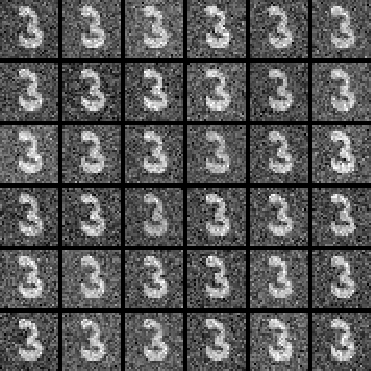
\includegraphics[width=\linewidth]{figs/Fig_single_chain_grid_beta2000.pdf}\\[-2pt]
\small (a) $\beta{=}2000$, SNR$=0.113$\\local endpoints ($\bar{\mathcal{D}}{=}0.282$)
\end{minipage}
\hfill
\begin{minipage}[t]{0.31\textwidth}
\centering
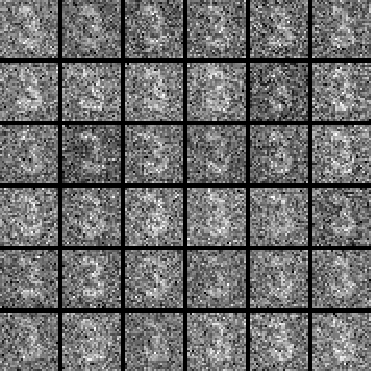
\includegraphics[width=\linewidth]{figs/Fig_single_chain_grid_beta200.pdf}\\[-2pt]
\small (b) $\beta{=}200$, SNR$=0.036$\\broader endpoints ($\bar{\mathcal{D}}{=}0.796$)
\end{minipage}
\hfill
\begin{minipage}[t]{0.31\textwidth}
\centering
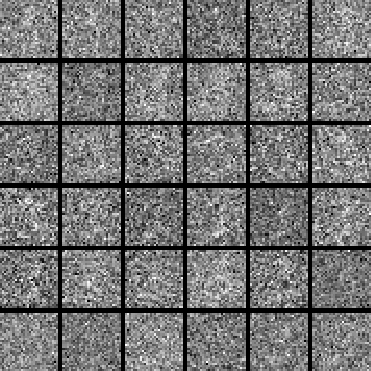
\includegraphics[width=\linewidth]{figs/Fig_single_chain_grid_beta50.pdf}\\[-2pt]
\small (c) $\beta{=}50$, SNR$=0.018$\\diffuse ($\bar{\mathcal{D}}{=}0.967$)
\end{minipage}
\caption{Single-chain endpoint grids from one digit-3 warm start. At
$\beta=2000$ the retained states remain local; decreasing $\beta$ broadens the
trajectory and eventually removes recognizable digit structure. Basin changes
describe finite-time dynamics, not increased expressiveness of the stationary
model.}
\label{fig:generation-regimes}
\end{figure}

\begin{figure}[ht]
\centering
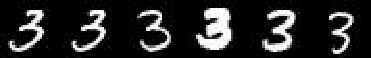
\includegraphics[width=0.55\textwidth]{figs/Fig_mnist_trajectory.pdf}\\[0.4em]
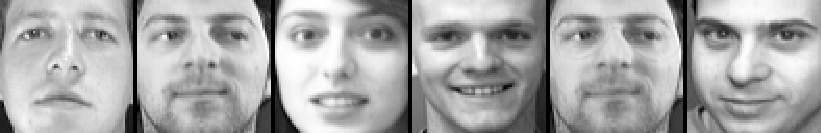
\includegraphics[width=0.95\textwidth]{figs/Fig_olivetti_trajectory_v2.pdf}

\small
\makebox[0.95\textwidth]{\centering $T = 0,\, 1000,\, 5000,\, 10000,\, 25000,\, 50000$\ \ (MNIST, top); $T = 0,\, 100,\, 500,\, 1000,\, 2000,\, 3000$\ \ (Olivetti, bottom)}
\caption{Chain snapshots without burn-in. Top: a digit-3 ULA trajectory at
$\beta=50$, shown after the denoising readout; its nearest-memory labels
change across checkpoints. Bottom: an unconditional Olivetti trajectory at
$\beta_{\mathrm{chain}}=200$ whose readout changes subjects. These examples
show finite-trajectory basin-label changes, not a quantitative mixing-time
estimate.}
\label{fig:trajectories}
\end{figure}

\subsection{Additional PF00076 diagnostics}
The following table and entropy figure document the full preprocessing and
decoder behavior beyond Figure~\ref{fig:protein} in the main text. All
comparisons use the same 68 sequences for fitting and evaluation. They are
therefore in-sample distributional diagnostics, and the profile-HMM pass rate
is saturated across methods.
\begin{table}[ht]
\centering
\caption{PF00076 endpoint statistics ($K=68$, $L=71$, $d=59$
after PCA). SeqID is maximum sequence identity to a stored sequence and KL is
amino-acid composition divergence. All reference statistics are in-sample;
$^\dagger$energy is evaluated under the Hopfield target at $\beta=8$.}
\label{tab:protein}
\small
\setlength{\tabcolsep}{4pt}
\resizebox{\textwidth}{!}{%
\begin{tabular}{@{}lccccc@{}}
\toprule
Method & $\mathcal{N}$ & $\bar{\mathcal{D}}$ & $\bar{E}$ & SeqID & KL \\
\midrule
Bootstrap (replay)          & $0.000 \pm 0.000$ & $1.000 \pm 0.012$ & $-0.500 \pm 0.000$ & $0.645 \pm 0.004$ & 0.133 \\
Gaussian perturbation       & $0.008 \pm 0.000$ & $1.002 \pm 0.007$ & $-0.492 \pm 0.000$ & $0.633 \pm 0.006$ & 0.132 \\
Random convex combination   & $0.510 \pm 0.009$ & $0.994 \pm 0.009$ & $-0.068 \pm 0.001$ & $0.562 \pm 0.000$ & 2.091 \\
GMM-PCA ($r{=}50$, $C{=}10$) & $0.606 \pm 0.009$ & $1.000 \pm 0.007$ & $+0.077 \pm 0.009$ & $0.540 \pm 0.003$ & 0.731 \\
VAE (latent${=}8$)          & $0.621 \pm 0.007$ & $0.834 \pm 0.022$ & $+0.118 \pm 0.007$ & $0.532 \pm 0.003$ & 0.416 \\
MALA ($\beta{=}77$)         & $0.249 \pm 0.004$ & $0.992 \pm 0.007$ & $-0.115 \pm 0.005$ & $0.609 \pm 0.012$ & 0.112 \\
ULA ($\beta{=}77$) & $0.243 \pm 0.004$ & $0.991 \pm 0.007$ & $-0.120 \pm 0.006$ & $0.616 \pm 0.012$ & 0.107 \\
ULA ($\beta{=}8$) & $0.623 \pm 0.006$ & $1.001 \pm 0.006$ & $3.08 \pm 0.06^\dagger$ & $0.538 \pm 0.006$ & 0.060 \\
\bottomrule
\end{tabular}}
\end{table}

\begin{figure}[ht]
\centering

\includegraphics[width=0.55\textwidth]{figs/Fig_protein_entropy_curve.pdf}
\caption{Responsibility entropy $H(\beta)/\log K$ for the PF00076 memory
($K=68$, $d=59$). The empirical inflection and the random spherical-memory
heuristic are shown for reference. Their difference reflects structured,
non-random memory geometry; the inflection is not an automatic quality-optimal
temperature.}
\label{fig:protein-entropy}
\end{figure}

\subsection{Financial log-return illustration}
The finance experiment is an exploratory application of finite-time
stochastic dynamics. Marginal affine correction and warm-started sequential
sampling are application-specific postprocessing choices, so these results do
not establish general generative superiority or follow from the exact-mixture
identity alone.
\begin{figure}[ht]
\centering

\includegraphics[width=0.95\textwidth]{figs/Fig_finance_qq_plots.pdf}
\caption{QQ plots of generated (after per-ticker affine correction) vs.\ historical log returns for five representative S\&P~500 constituents. Quantiles track closely for these tickers; $64.2\%$ of all $424$ tickers pass the two-sample KS test at the $5\%$ level. The dashed red line is $y=x$.}
\label{fig:finance-qq}
\end{figure}

\begin{figure}[ht]
\centering

\includegraphics[width=0.45\textwidth]{figs/Fig_finance_correlation.pdf}
\caption{Pairwise correlation: historical vs.\ generated. Each point represents one of $89{,}676$ asset pairs. The scatter around $y=x$ shows partial preservation of cross-asset dependence structure (Frobenius error $26.3\%$ vs.\ $15.6\%$ for bootstrap).}
\label{fig:finance-correlation}
\end{figure}

\begin{figure}[ht]
\centering

\includegraphics[width=0.75\textwidth]{figs/Fig_finance_tail_survival.pdf}
\caption{Empirical survival functions of historical and generated
equal-weighted portfolio returns. Right and left tails are displayed together
on a log scale for descriptive comparison.}
\label{fig:finance-tails}
\end{figure}

\begin{table}[ht]
\centering
\caption{Finance summary. Distributional rows use an i.i.d. endpoint
pool followed by per-ticker affine correction; temporal rows use a separate
warm-started sequential MALA protocol. These application-specific pipelines
are not an equilibrium validation or a cross-model quality ranking.}
\label{tab:finance-summary}
\small
\begin{tabular}{@{}lll@{}}
\toprule
Property & SA (corrected) & Bootstrap \\
\midrule
\multicolumn{3}{@{}l@{}}{\textit{Distributional fidelity (i.i.d.\ pool, 900 samples)}} \\
KS $p$-value (mean; 64.2\% pass at $5\%$) & 0.193 & 0.622 \\
Cross-asset Frobenius error & 26.3\% & 15.6\% \\
Novelty ($1-\max_k\cos$) & $0.768\pm0.001$ & 0.000 \\
\multicolumn{3}{@{}l@{}}{\textit{Temporal properties (MALA warm-start, 2766 days)}} \\
SF2: Return unpredictability & Reproduced [ACF($g$) in 99\% CI, $\beta{=}12$] & N/A \\
SF3: Volatility clustering & Not reproduced ($\beta{=}12$) & N/A \\
\bottomrule
\end{tabular}
\end{table}

\begin{figure}[ht]
\centering

\includegraphics[width=0.95\textwidth]{figs/Fig_finance_return_acf.pdf}\\[4pt]

\includegraphics[width=0.95\textwidth]{figs/Fig_finance_vol_clustering.pdf}
\caption{Stylized Facts~2 and~3: Autocorrelation analysis for five S\&P~500 tickers.
\textbf{Top row}: ACF($g$): the generated series (blue) stays within the 99\% confidence band (dashed) at all lags, matching the near-zero autocorrelation of historical returns (red).
\textbf{Bottom row}: ACF($g^2$): the historical series (red) shows persistent positive autocorrelation characteristic of volatility clustering, while the generated series (blue) shows ACF($g^2$) $\approx 0$ under this stationary sequential protocol.}
\label{fig:finance-acf-combined}
\end{figure}

\subsection{Olivetti masking diagnostics}
The Olivetti tables quantify memory-subset restriction. Hard masking
sets off-subject component weights to zero, so high subject recovery is expected
from the restricted support; the experiment remains useful for measuring
leakage and the geometric effect of soft biases.
\begin{table}[ht]
\centering
\caption{Subject-recovery rate on Olivetti faces ($K=100$,
$d=4096$, 10 subjects). The hard mask removes all off-subject components;
unconditional recovery is near the uniform 10-subject rate. The protocols use
different endpoint allocations as detailed in the text.}
\label{tab:olivetti-recovery}
\small
\begin{tabular}{@{}lc@{}}
\toprule
Regime & Subject-recovery rate \\
\midrule
Random guess (uniform over 10 subjects) & $0.100$ \\
Unconditional SA, uniform warm-start    & $0.104$ \\
Hard-masked ULA ($b_{k}{=}-\infty$ off-subject) & $0.960$ \\
\bottomrule
\end{tabular}
\end{table}

\begin{table}[ht]
\centering
\caption{Single-$\beta$ masked sweep on Olivetti subject 0, with
20 chains per row. Novelty is median minimum cosine distance to an in-subject
memory; hit rate uses the nearest-mean rule.}
\label{tab:olivetti-betasweep}
\small
\begin{tabular}{@{}lcccccc@{}}
\toprule
$\beta$ & $2$ & $8$ & $32$ & $128$ & $512$ & $2048$ \\
\midrule
Novelty & $0.009$ & $0.009$ & $0.006$ & $0.005$ & $0.000$ & $0.000$ \\
Hit rate & $1.000$ & $1.000$ & $0.950$ & $0.900$ & $0.900$ & $0.900$ \\
\bottomrule
\end{tabular}
\end{table}

\section{Baseline Method Specifications}\label{app:baseline-methods}
% ─────────────────────────────────────────────────────────────────────────────

Complete mathematical specifications for the two learned generative
baselines (GMM-PCA and the VAE; Table~\ref{tab:mnist-baselines}) follow.
All hyperparameters reported here were used without modification in the experiments;
the implementation is publicly available in \texttt{code/mnist-experiment/} and
\texttt{code/vae-experiment/} in the accompanying repository.

% ── GMM-PCA ──────────────────────────────────────────────────────────────────
\subsection{GMM-PCA}\label{app:gmm-pca}

\paragraph{Dimensionality reduction.}
Let $\mathbf{X}\in\mathbb{R}^{d\times K}$ be the column-normalized memory matrix
($d{=}784$, $K{=}100$). Compute the economy SVD
$\mathbf{X}=\mathbf{U}\boldsymbol{\Sigma}\mathbf{V}^{\!\top}$ and retain the top
$r{=}50$ left singular vectors, forming $\mathbf{U}_{r}\in\mathbb{R}^{d\times r}$.
Project each stored pattern to a low-dimensional code:
$\mathbf{z}_{k}=\mathbf{U}_{r}^{\!\top}\mathbf{m}_{k}\in\mathbb{R}^{r}$, $k=1,\dots,K$.
For the digit ``3'' memory matrix, the top 50 components capture $>$95\% of total variance.

\paragraph{Gaussian mixture model.}
Fit a $C{=}10$ component GMM with \emph{diagonal} covariance to the code matrix
$\mathbf{Z}{=}[\mathbf{z}_1|\cdots|\mathbf{z}_K]\in\mathbb{R}^{r\times K}$ via
Expectation-Maximization~\cite{dempsterMaximumLikelihoodIncomplete1977}:
\begin{equation}
  p(\mathbf{z}) = \sum_{c=1}^{C}\pi_c\,
  \mathcal{N}\!\bigl(\mathbf{z};\,\boldsymbol{\mu}_c,\,\mathrm{diag}(\boldsymbol{\sigma}_c^2)\bigr),
  \quad \sum_{c=1}^{C}\pi_c=1,\quad \pi_c\geq 0.
\end{equation}
Parameters $\{\pi_c,\boldsymbol{\mu}_c,\boldsymbol{\sigma}_c^2\}_{c=1}^{C}$ are estimated
by EM with K-means$\texttt{++}$ initialization and convergence tolerance $10^{-8}$ on the
log-likelihood.
The diagonal-covariance constraint reduces the number of covariance parameters
and assumes conditionally independent PCA coordinates within each component.
The implementation also floors every fitted coordinate variance at $10^{-6}$;
this explicit floor, rather than the diagonal form alone, prevents zero-variance
coordinates from making a component singular.

\paragraph{Sampling.}
To draw one sample: (i) sample component $c\sim\mathrm{Categorical}(\boldsymbol{\pi})$;
(ii) sample $\tilde{\mathbf{z}}\sim\mathcal{N}(\boldsymbol{\mu}_c,\mathrm{diag}(\boldsymbol{\sigma}_c^2))$;
(iii) reconstruct $\hat{\boldsymbol{\xi}}=\mathbf{U}_{r}\tilde{\mathbf{z}}$ and
renormalize to unit $\ell_2$ norm.
The 150 evaluation samples are drawn i.i.d.\ under this procedure with a fixed seed.

\paragraph{Hyperparameters.}
$r{=}50$ PCA components; $C{=}10$ GMM components; K-means$\texttt{++}$ initialization;
EM convergence tolerance $10^{-8}$; coordinate-variance floor $10^{-6}$.

% ── VAE ──────────────────────────────────────────────────────────────────────
\subsection{Variational Autoencoder}\label{app:vae}

\paragraph{Architecture.}
The encoder maps $\mathbf{x}\in\mathbb{R}^{784}$ to the parameters of an approximate posterior:
\begin{align}
  \mathbf{h}_1 &= \mathrm{ReLU}(\mathbf{W}_1\mathbf{x}+\mathbf{b}_1),\quad
    \mathbf{W}_1\in\mathbb{R}^{256\times 784}, \\
  \mathbf{h}_2 &= \mathrm{ReLU}(\mathbf{W}_2\mathbf{h}_1+\mathbf{b}_2),\quad
    \mathbf{W}_2\in\mathbb{R}^{128\times 256}, \\
  \boldsymbol{\mu}_\phi(\mathbf{x}) &= \mathbf{W}_\mu\mathbf{h}_2+\mathbf{b}_\mu,\quad
    \mathbf{W}_\mu\in\mathbb{R}^{8\times 128}, \\
  \log\boldsymbol{\sigma}^2_\phi(\mathbf{x}) &= \mathbf{W}_\sigma\mathbf{h}_2+\mathbf{b}_\sigma,\quad
    \mathbf{W}_\sigma\in\mathbb{R}^{8\times 128}.
\end{align}
The decoder is architecturally symmetric: $8\to128\to256\to784$, with ReLU activations on
hidden layers and a linear output.
All weight matrices are Glorot-uniform initialized; biases are zero-initialized.
The decoder output is renormalized to unit $\ell_2$ norm before computing metrics, matching
the normalization convention of all other methods in Table~\ref{tab:mnist-baselines}.

\paragraph{Objective.}
We minimize the $\beta$-VAE objective~\cite{higginsBetaVAELearningBasic2017}:
\begin{equation}
  \mathcal{L}(\phi,\theta;\mathbf{x})
  = \underbrace{\bigl\lVert\mathbf{x}-\hat{\mathbf{x}}_\theta(\mathbf{z})\bigr\rVert_2^2}
    _{\text{reconstruction}}
  +\; \beta_{\mathrm{KL}}\underbrace{D_{\mathrm{KL}}\!\bigl(
    q_\phi(\mathbf{z}|\mathbf{x})\,\big\|\,\mathcal{N}(\mathbf{0},\mathbf{I})\bigr)}
    _{\text{regularization}},
\label{eq:vae-elbo}
\end{equation}
where $q_\phi(\mathbf{z}|\mathbf{x})=\mathcal{N}(\boldsymbol{\mu}_\phi(\mathbf{x}),
\mathrm{diag}(\boldsymbol{\sigma}^2_\phi(\mathbf{x})))$ and the reparameterization trick
$\mathbf{z}=\boldsymbol{\mu}_\phi(\mathbf{x})+\boldsymbol{\sigma}_\phi(\mathbf{x})\odot
\boldsymbol{\epsilon}$, $\boldsymbol{\epsilon}\sim\mathcal{N}(\mathbf{0},\mathbf{I})$,
enables gradient flow through the sampling step.
The KL term has a closed form:
\begin{equation}
  D_{\mathrm{KL}} = \tfrac{1}{2}\sum_{j=1}^{8}\bigl[
    \mu_{\phi,j}^2+\sigma_{\phi,j}^2 - \log\sigma_{\phi,j}^2 - 1\bigr].
\end{equation}

\paragraph{Two-phase training protocol.}
In preliminary runs on this $K=100$ dataset, training directly with the full
$\beta$-VAE objective produced posterior-collapse symptoms: the encoder used
little of the latent code and the decoder approached a nearly constant map. We
therefore used a two-phase schedule. The warm-up phase (epochs 1--2{,}000)
trained with $\beta_{\mathrm{KL}}=0$, which established a non-degenerate
reconstruction map before regularization. The fine-tuning phase (epochs
2{,}001--4{,}000) increased the KL weight linearly from zero to
$\beta_{\mathrm{KL}}=0.0001$. Annealing the KL weight is a standard response to
posterior collapse~\cite{lucasHowAvoidTrivial2019}; this experiment does not
support a general claim about when collapse occurs as dataset size changes.

\paragraph{Optimization and sampling.}
Optimizer: Adam~\cite{kingmaAdamMethodStochastic2014} with learning rate $10^{-3}$,
$\beta_1{=}0.9$, $\beta_2{=}0.999$, $\varepsilon{=}10^{-8}$, batch size $K{=}100$
(full-dataset batches throughout).
No weight decay, dropout, or data augmentation was applied.
At evaluation time, 150 samples are drawn by sampling
$\mathbf{z}\sim\mathcal{N}(\mathbf{0},\mathbf{I}_8)$ and decoding
$\hat{\mathbf{x}}=\hat{\mathbf{x}}_\theta(\mathbf{z})$, then renormalizing to unit norm.

\paragraph{Hyperparameter selection.}
The final configuration (latent dimension 8,
$\beta_{\mathrm{KL}}=0.0001$) was chosen by a grid search over latent
dimension $\in\{4,8,16,32\}$ and
$\beta_{\mathrm{KL}}\in\{0.1,0.01,0.001,0.0001\}$, using novelty and diversity
computed against the same 100-image reference set. This was not an independent
held-out validation procedure.
Latent dimension 8 with $\beta_{\mathrm{KL}}=0.0001$ produced
$\mathcal{N}=0.214\pm0.005$ and $\bar{\mathcal{D}}=0.441\pm0.008$ under the
descriptive metrics. Smaller latent dimensions, larger KL weights,
and the latent-32 setting with $\beta_{\mathrm{KL}}=0.01$ produced less endpoint
spread. These observations document hyperparameter sensitivity; they are not a
quality ranking against the Hopfield target.

% ── DDPM ────────────────────────────────────────────────────────────────────
\subsection{Denoising diffusion protocol}\label{app:ddpm}

The diffusion diagnostic used a denoising diffusion probabilistic model
(DDPM)~\cite{hoDenoisingDiffusionProbabilistic2020} on the same flattened,
unit-normalized MNIST vectors as the other image experiments. Because the input
was represented as a vector rather than a two-dimensional image, the denoiser
was an MLP rather than a convolutional U-Net. At step $t$, it concatenated
$\mathbf x_t\in\mathbb R^{784}$ with a 64-dimensional sinusoidal time
embedding and passed the result through layers of widths
$848\to512\to256\to512\to784$, with ReLU activations on the hidden layers.
The output estimated the added noise.

The forward process used $T=200$ steps and a linear variance schedule from
$\beta_1=10^{-4}$ to $\beta_T=0.02$. With
$\bar\alpha_t=\prod_{s=1}^t(1-\beta_s)$, its marginal transition was:
\begin{equation}
q(\mathbf x_t\mid\mathbf x_0)
=\mathcal N\!\left(\sqrt{\bar\alpha_t}\,\mathbf x_0,
(1-\bar\alpha_t)\mathbf I\right).
\end{equation}
Training used Adam with learning rate $10^{-3}$ and full-dataset batches. Each
update sampled a time for each input, added the corresponding Gaussian noise,
and minimized the squared error between the added noise and the network output.
The $K=100$ run used 5,000 epochs.

Sampling began at $\mathbf x_T\sim\mathcal N(\mathbf0,\mathbf I)$ and applied
the standard reverse update:
\begin{equation}
\mathbf x_{t-1}=\frac{1}{\sqrt{\alpha_t}}
\left(\mathbf x_t-
\frac{\beta_t}{\sqrt{1-\bar\alpha_t}}
\widehat{\boldsymbol\epsilon}_{\theta}(\mathbf x_t,t)\right)
+\sqrt{\beta_t}\,\mathbf z,
\end{equation}
where $\mathbf z$ was standard Gaussian except at the final step. Outputs were
normalized to unit $\ell_2$ norm before the geometric diagnostics were
computed.

Under this particular protocol, the $K=100$ run produced novelty $0.938$,
diversity $0.991$, and mean nearest-memory cosine $0.062$. These values were
close to the isotropic-noise diagnostic, and the training loss plateaued near
$0.855$. The result identifies a failure of this flattened-vector MLP protocol;
it does not establish a general comparison with diffusion models. A
convolutional architecture, a representation adapted to images, a tuned noise
schedule, and matched optimization compute could change the outcome.


\section{Finite-Step Sensitivity Analyses}
These finite-step diagnostics do not establish mixing or unbiasedness. The
Gaussian control used $\sqrt{2\alpha/\beta}$, not the exact component scale
$\beta^{-1/2}$.
\begin{table}[ht]
\centering
\caption{Step-size sweep on MNIST digit 3 ($K=100$, $d=784$,
$\beta=2000$). The ULA and MALA endpoint summaries are close at small $\alpha$ in
this finite protocol. This agreement and high acceptance do not establish
mixing or bound ULA bias.}
\label{tab:stepsize-sweep}
\small
\begin{tabular}{@{}rcccccc@{}}
\toprule
$\alpha$ & Accept & \multicolumn{2}{c}{Novelty} & \multicolumn{2}{c}{Diversity} & $\Delta E$ \\
 & rate & ULA & MALA & ULA & MALA & (ULA$-$MALA) \\
\midrule
0.001 & $>$0.99 & 0.151 & 0.150 & 0.595 & 0.595 & $<$0.001 \\
0.005 & $>$0.99 & 0.151 & 0.151 & 0.599 & 0.597 & $<$0.001 \\
0.01  & 0.992 & 0.152 & 0.151 & 0.600 & 0.598 & 0.002 \\
0.02  & 0.978 & 0.153 & 0.151 & 0.600 & 0.598 & 0.003 \\
0.05  & 0.911 & 0.155 & 0.151 & 0.602 & 0.598 & 0.006 \\
0.1   & 0.747 & 0.158 & 0.151 & 0.605 & 0.597 & 0.011 \\
0.2   & 0.000 & 0.165 & 0.000 & 0.612 & 0.000 & --- \\
0.3   & 0.000 & 0.172 & 0.000 & 0.619 & 0.000 & --- \\
0.5   & 0.000 & 0.189 & 0.000 & 0.635 & 0.000 & --- \\
\bottomrule
\end{tabular}
\end{table}

\begin{table}[ht]
\centering
\caption{Gaussian controls on MNIST digit 3 at $\beta=200$.
FD$_{\text{diag}}$ is the diagonal pixel-space Fr\'{e}chet distance to stored
patterns. The moment-matched controls differ from exact component-conditioned
Gaussian sampling, which is reported in the main text.}
\label{tab:noise-control}
\small
\begin{tabular}{@{}lccccc@{}}
\toprule
Method & $\mathcal{N}$ & $\bar{\mathcal{D}}$ & $\bar{E}$ & Max-$\cos$ & FD$_{\text{diag}}$ \\
\midrule
Stored patterns                   & 0.000 & 0.459 & $-0.50$ & 1.000 & ---  \\
ULA ($\beta{=}200$)       & 0.547 & 0.885 & $+1.47$ & 0.453 & 2.81 \\
Gaussian (matched $\mu,\sigma^2$) & 0.672 & 0.878 & $+1.78$ & 0.328 & 2.86 \\
Gaussian (isotropic)              & 0.943 & 1.000 & $+2.34$ & 0.057 & 3.91 \\
\bottomrule
\end{tabular}
\end{table}

\begin{figure}[ht]
\centering
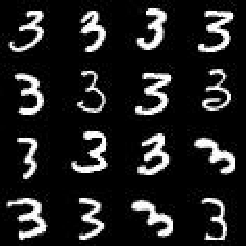
\includegraphics[width=0.19\textwidth]{figs/Fig_noise_control_stored.pdf}%
\hfill
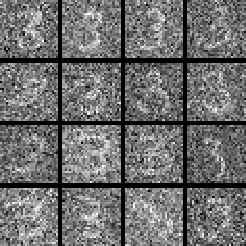
\includegraphics[width=0.19\textwidth]{figs/Fig_noise_control_sa_beta200.pdf}%
\hfill
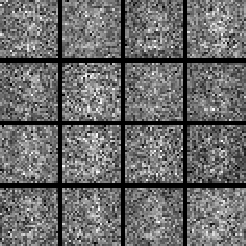
\includegraphics[width=0.19\textwidth]{figs/Fig_noise_control_gauss_matched.pdf}%
\hfill
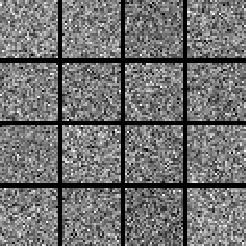
\includegraphics[width=0.19\textwidth]{figs/Fig_noise_control_gauss_iso.pdf}%
\hfill
\IfFileExists{figs/Fig_noise_control_maxcos_hist.pdf}{%
  
\includegraphics[width=0.19\textwidth]{figs/Fig_noise_control_maxcos_hist.pdf}%
}{%
  \framebox[0.19\textwidth]{\rule{0pt}{3cm}\small hist}%
}

\small
\makebox[0.19\textwidth]{\centering (a) Stored}%
\hfill
\makebox[0.19\textwidth]{\centering (b) SA ($\beta{=}200$)}%
\hfill
\makebox[0.19\textwidth]{\centering (c) Gauss (matched)}%
\hfill
\makebox[0.19\textwidth]{\centering (d) Gauss (iso)}%
\hfill
\makebox[0.19\textwidth]{\centering (e) Max-$\cos$ dist.}
\caption{Gaussian-control images. Panels show stored patterns, ULA
endpoints at $\beta=200$, a marginal moment-matched Gaussian, an isotropic
norm-matched Gaussian, and nearest-memory cosine distributions. These controls
do not condition Gaussian noise on a sampled memory and therefore are not the
exact Hopfield-mixture baseline.}
\label{fig:noise-control}
\end{figure}

\begin{table}[H]
\centering
\caption{ULA and MALA endpoint summaries over $\beta$; $\Delta$
columns report ULA minus MALA. Small differences under this protocol are
descriptive and do not prove convergence or absence of ULA bias.}
\label{tab:mala-generation}
\small
\begin{tabular}{@{}rccccccc@{}}
\toprule
$\beta$ & Accept & $\mathcal{N}_{\text{SA}}$ & $\Delta\mathcal{N}$ & $\bar{\mathcal{D}}_{\text{SA}}$ & $\Delta\bar{\mathcal{D}}$ & $\bar{E}_{\text{SA}}$ & $\Delta\bar{E}$ \\
\midrule
200  & 99.2\% & 0.548 & $+0.002$ & 0.885 & $+0.002$ & $+1.467$ & $+0.018$ \\
500  & 99.2\% & 0.375 & $+0.002$ & 0.782 & $+0.002$ & $+0.287$ & $+0.007$ \\
1000 & 99.2\% & 0.251 & $+0.002$ & 0.687 & $+0.002$ & $-0.107$ & $+0.004$ \\
\bottomrule
\end{tabular}
\end{table}

\section{Data-Scale Diagnostic: Stochastic Attention and DDPM}\label{app:scaling}

We also varied the number of digit-3 images over
$K\in\{100,500,1000,2000,3500\}$. For stochastic attention, the diagnostic
temperature $\beta^*$ was the point of maximum absolute slope in the empirical
responsibility-entropy curve over the scanned grid; a second condition used
$5\beta^*$. This construction gives a reproducible temperature rule for the
table, but it is not guaranteed to optimize perceptual quality or define a
phase transition. The DDPM architecture and schedule remained those in
Appendix~\ref{app:ddpm}; its epoch count decreased from 5,000 at $K=100$ to
1,000 at $K=3500$ to keep the number of full-batch updates in the same order.

\begin{table}[ht]
\centering
\caption{Digit-3 data-scale diagnostic. MaxCos is mean cosine similarity to
the nearest reference image. Novelty and diversity are geometric spread
statistics. The table compares the specified protocols, not the best possible
implementation of either model family.}
\label{tab:scaling}
\small
\resizebox{\textwidth}{!}{%
\begin{tabular}{@{}rrccccccccc@{}}
\toprule
$K$ & $K/d$ & $\beta^*$ & \multicolumn{3}{c}{ULA ($\beta=\beta^*$)} &
\multicolumn{3}{c}{ULA ($\beta=5\beta^*$)} & \multicolumn{2}{c}{DDPM} \\
\cmidrule(lr){4-6}\cmidrule(lr){7-9}\cmidrule(lr){10-11}
 & & & $\mathcal N$ & $\bar{\mathcal D}$ & MaxCos &
$\mathcal N$ & $\bar{\mathcal D}$ & MaxCos & MaxCos & Train (s) \\
\midrule
100  & 0.13 & 9  & 0.874 & 0.993 & 0.126 & 0.763 & 0.969 & 0.237 & 0.061 & 34 \\
500  & 0.64 & 13 & 0.851 & 0.991 & 0.149 & 0.722 & 0.955 & 0.278 & 0.073 & 37 \\
1000 & 1.28 & 15 & 0.839 & 0.989 & 0.161 & 0.697 & 0.949 & 0.303 & 0.078 & 46 \\
2000 & 2.55 & 18 & 0.827 & 0.987 & 0.173 & 0.673 & 0.940 & 0.327 & 0.086 & 66 \\
3500 & 4.46 & 18 & 0.825 & 0.987 & 0.175 & 0.673 & 0.944 & 0.327 & 0.090 & 75 \\
\bottomrule
\end{tabular}}
\end{table}

\begin{figure}[ht]
\centering

\includegraphics[width=0.95\textwidth]{figs/Fig_scaling_sa_vs_ddpm.pdf}
\caption{Data-scale diagnostic on MNIST digit 3. The panels show
nearest-memory cosine, novelty, diversity, and the empirical entropy-slope
temperature $\beta^*$. The DDPM curve describes the flattened-vector MLP in
Appendix~\ref{app:ddpm}; it is not a benchmark against modern image diffusion
systems.}
\label{fig:scaling}
\end{figure}

Within these protocols, ULA nearest-memory cosine increased with $K$, whereas
the DDPM diagnostic remained near the isotropic-noise value over the tested
range. The comparison is confounded by representation, architecture, noise
schedule, and compute allocation. It therefore supports the narrower claim
that the analytic Hopfield score worked without training in this low-data
setup, not that stochastic attention generally outperforms diffusion.

\section{VAE Data-Scale Sensitivity}
The following table documents the data-scale experiment. Because
the evaluation uses nearest-memory geometry and the Hopfield model's own energy,
it does not establish model-quality superiority.
\begin{table}[ht]
\centering
\caption{Comparison of SA against VAEs trained on $10{\times}$ to $100{\times}$ more data. All metrics computed against the same $K{=}100$ digit-3 memory matrix. MaxCos: mean max-cosine similarity to nearest stored pattern. On-manif: fraction of samples with Hopfield energy $E<0$.}
\label{tab:full-vae}
\small
\begin{tabular}{@{}llccccc@{}}
\toprule
Method & Train data & MaxCos & $\mathcal{N}$ & $\bar{\mathcal{D}}$ & $\bar{E}$ & On-manif \\
\midrule
VAE (lat${=}8$, original)  & $K{=}100$ & $0.775$ & $0.225$ & $0.426$ & $-0.276$ & $100\%$ \\
VAE-D3 (lat${=}8$)         & $N{=}1{,}000$ & $0.668$ & $0.332$ & $0.603$ & $-0.168$ & $94\%$ \\
VAE-D3 (lat${=}32$)        & $N{=}1{,}000$ & $0.743$ & $0.257$ & $0.466$ & $-0.244$ & $100\%$ \\
VAE-D3 (lat${=}64$)        & $N{=}1{,}000$ & $0.762$ & $0.238$ & $0.413$ & $-0.263$ & $100\%$ \\
VAE-all (lat${=}32$, top)  & $N{=}10{,}000$ & $0.830$ & $0.170$ & $0.325$ & $-0.330$ & $100\%$ \\
\midrule
ULA ($\beta{=}2000$) & $K{=}100$ & $0.848$ & $0.152$ & $0.600$ & $-0.303$ & $100\%$ \\
ULA ($\beta{=}200$)          & $K{=}100$ & $0.452$ & $0.548$ & $0.885$ & $+1.467$ & $0\%$ \\
\bottomrule
\end{tabular}
\end{table}

\section{Principal Component Analysis}\label{app:pca}
% ═══════════════════════════════════════════════════════════════════════════════

Several experiments use Principal Component Analysis (PCA): the protein
pipeline projects one-hot encodings from $\mathbb{R}^{1420}$ to
$\mathbb{R}^{59}$, and the GMM-PCA baseline operates in a 50-dimensional
subspace. We summarize the construction for completeness.

\paragraph{Setup.}
Given a memory matrix $\mathbf{X} = [\mathbf{m}_1,\dots,\mathbf{m}_K] \in \mathbb{R}^{d \times K}$, define the column mean $\bar{\mathbf{m}} = \frac{1}{K}\sum_{k=1}^{K}\mathbf{m}_k$ and the centered matrix $\tilde{\mathbf{X}} = \mathbf{X} - \bar{\mathbf{m}}\mathbf{1}_K^\top \in \mathbb{R}^{d \times K}$.

\paragraph{Singular value decomposition.}
The centered matrix has the following economy SVD:
\begin{equation}\label{eq:pca-svd}
    \tilde{\mathbf{X}} = \mathbf{U}\boldsymbol{\Sigma}\mathbf{V}^\top,
\end{equation}
where $\mathbf{U} \in \mathbb{R}^{d \times r}$ has orthonormal columns (the \emph{principal directions}), $\boldsymbol{\Sigma} = \operatorname{diag}(\sigma_1,\dots,\sigma_r)$ with $\sigma_1 \ge \sigma_2 \ge \cdots \ge \sigma_r > 0$ (the \emph{singular values}), and $\mathbf{V} \in \mathbb{R}^{K \times r}$ has orthonormal columns. Here $r = \operatorname{rank}(\tilde{\mathbf{X}}) \le \min(d, K)$.

\paragraph{Variance interpretation.}
The $j$-th principal component of pattern $\mathbf{m}_k$ is $z_{kj} = \mathbf{u}_j^\top(\mathbf{m}_k - \bar{\mathbf{m}})$. The variance of the $j$-th component across the $K$ patterns is $\sigma_j^2 / K$. The first $p$ components capture the following fraction of total variance:
\begin{equation}\label{eq:pca-variance}
    \rho(p) = \frac{\sum_{j=1}^{p}\sigma_j^2}{\sum_{j=1}^{r}\sigma_j^2}.
\end{equation}

\paragraph{Projection and reconstruction.}
To reduce dimensionality from $d$ to $p \le r$, define the projection matrix $\mathbf{W}_p = \mathbf{U}_{:,1:p}^\top \in \mathbb{R}^{p \times d}$ using the first $p$ principal directions. The projected representation of pattern $\mathbf{m}_k$ is $\mathbf{z}_k = \mathbf{W}_p(\mathbf{m}_k - \bar{\mathbf{m}}) \in \mathbb{R}^p$, and the approximate reconstruction is $\hat{\mathbf{m}}_k = \bar{\mathbf{m}} + \mathbf{W}_p^\top\mathbf{z}_k$. Among all rank-$p$ linear projections, PCA minimizes the mean squared reconstruction error $\frac{1}{K}\sum_{k=1}^{K}\|\mathbf{m}_k - \hat{\mathbf{m}}_k\|_2^2 = \frac{1}{K}\sum_{j=p+1}^{r}\sigma_j^2$.

\paragraph{Usage in this paper.}
In the protein experiment (Appendix~\ref{app:protein-protocol}), we select $p$
such that $\rho(p)\geq0.95$, yielding $p=59$ from $d=1420$. After projection,
the representations are $\ell_2$-normalized to form the memory matrix.

% ═══════════════════════════════════════════════════════════════════════════════

\section{Scoped Multi-Head Stochastic Attention}
\label{app:multihead}

We retain the multi-head construction with its state spaces and output map made
explicit. This is a product of tied-key/value stochastic-attention heads, not a
claim that an arbitrary transformer head possesses a scalar energy.

Let $\bar{\mathbf m}$ be the memory mean. For head $h=1,\ldots,H$, let
$\mathbf P_h\in\mathbb R^{d_h\times d}$ have orthonormal rows, with the row
spaces of distinct heads mutually orthogonal. The head state is
$\mathbf z^{(h)}\in\mathbb R^{d_h}$ and its tied projected memories are
$\mathbf v_k^{(h)}=\mathbf P_h(\mathbf m_k-\bar{\mathbf m})$. Each head has
the following energy:
\begin{equation}
E_h(\mathbf z)=\frac12\lVert\mathbf z\rVert_2^2
-\frac1\beta\log\sum_{k=1}^K r_k^{(h)}
\exp\!\left(\beta\mathbf v_k^{(h)\top}\mathbf z\right).
\label{eq:multihead-energy}
\end{equation}
Independent Langevin chains target the product density
$p(\mathbf z^{(1)},\ldots,\mathbf z^{(H)})=\prod_h p_h(\mathbf z^{(h)})$.
The following linear reconstruction maps their concatenated output back to the
original space:
\begin{equation}
\widehat{\boldsymbol\xi}
=\bar{\mathbf m}+\sum_{h=1}^H\mathbf P_h^\top\mathbf z^{(h)}
=\bar{\mathbf m}+\mathbf W_O
[\mathbf z^{(1)};\ldots;\mathbf z^{(H)}],
\qquad
\mathbf W_O=[\mathbf P_1^\top\ \cdots\ \mathbf P_H^\top].
\label{eq:multihead-output}
\end{equation}
Equation~\eqref{eq:multihead-output} is deterministic postprocessing of the
product target. We do not assert that its pushforward has a Hopfield energy in
the reconstructed space. Because the head chains are independent, they may
select different memory components and thereby recombine subspace-level
features. A model requiring the same component index across heads would instead
need an explicitly coupled joint target.

\begin{algorithm}[H]
\caption{Independent-head Stochastic Attention}
\label{alg:multihead}
\begin{algorithmic}[1]
\REQUIRE Projections $\{\mathbf P_h\}_{h=1}^H$, memories $\mathbf X$,
head multiplicities $\{\mathbf r^{(h)}\}$, mean $\bar{\mathbf m}$, $\beta$,
$\alpha$, $T$, initial head states $\{\mathbf z_0^{(h)}\}$
\FOR{$h=1,\ldots,H$}
\STATE $\mathbf V_h\leftarrow\mathbf P_h
(\mathbf X-\bar{\mathbf m}\mathbf1^\top)$
\STATE Run Algorithm~\ref{alg:stochastic-attention} in $\mathbb R^{d_h}$
with memories $\mathbf V_h$, multiplicities $\mathbf r^{(h)}$, $C\equiv0$,
and $\lambda=0$ to obtain $\mathbf z_T^{(h)}$
\ENDFOR
\STATE $\widehat{\boldsymbol\xi}\leftarrow\bar{\mathbf m}
+\sum_h\mathbf P_h^\top\mathbf z_T^{(h)}$
\RETURN $\widehat{\boldsymbol\xi}$
\end{algorithmic}
\end{algorithm}

The proof-of-concept implementation used disjoint blocks of left singular
vectors for the $\mathbf P_h$. With $K=100$ digit-3 memories, the centered
matrix has rank at most 99. The code nevertheless requested the 100 left
singular vectors returned by the economy SVD, so the final direction
corresponded to a zero singular value rather than a nonzero principal
component. For $H=4$, the 100 returned directions were divided into four blocks
of 25. In addition, the implementation projected the uncentered memories and
normalized every projected memory before sampling, then added the mean during
reconstruction. Those choices differ from the idealized centered construction
in Algorithm~\ref{alg:multihead}. Table~\ref{tab:multihead} is therefore an
archived proof-of-concept, not a direct validation of the product target above.
Changing $H$ also changes the model and reconstruction, so the rows do not show
that more heads improve sampling from one fixed target.

\begin{table}[H]
\centering
\caption{PCA-partitioned multi-head proof-of-concept at $\beta=200$. Metrics
are computed against each configuration's own memory set. The implementation
differences from Algorithm~\ref{alg:multihead} are described in the text.}
\label{tab:multihead}
\small
\begin{tabular}{@{}llccc@{}}
\toprule
Configuration & $K$ & Novelty & Diversity & Max cosine \\
\midrule
SA ($H=1$) & 100  & $0.547\pm0.002$ & $0.885\pm0.002$ & $0.453\pm0.002$ \\
SA ($H=1$) & 500  & $0.548\pm0.003$ & $0.892\pm0.003$ & $0.452\pm0.003$ \\
SA ($H=1$) & 1000 & $0.548\pm0.002$ & $0.892\pm0.003$ & $0.452\pm0.002$ \\
\midrule
SA ($H=2$, 50 PCs/head) & 100 & $0.175\pm0.006$ & $0.307\pm0.002$ & $0.825\pm0.006$ \\
SA ($H=4$, 25 PCs/head) & 100 & $0.187\pm0.005$ & $0.291\pm0.002$ & $0.815\pm0.005$ \\
SA ($H=5$, 20 PCs/head) & 100 & $0.196\pm0.005$ & $0.263\pm0.002$ & $0.804\pm0.005$ \\
\midrule
SA ($H=4$, 25 PCs/head) & 500  & $0.391\pm0.003$ & $0.475\pm0.002$ & $0.609\pm0.003$ \\
SA ($H=4$, 25 PCs/head) & 1000 & $0.469\pm0.004$ & $0.582\pm0.003$ & $0.531\pm0.004$ \\
\bottomrule
\end{tabular}
\end{table}

For $H=4$ and $K=100$, the PCA blocks explain 81.2\%, 12.6\%, 4.5\%, and
1.6\% of the retained variance. The higher nearest-memory cosine in the
multi-head rows is consistent with lower-dimensional head states and the
deterministic PCA reconstruction, but it should not be attributed solely to
better Markov-chain mixing. Learned projections, coupled heads, and validation
inside an actual transformer remain open extensions.

% ═══════════════════════════════════════════════════════════════════════════════
